\section{Analysis}\label{sec:analysis}
The main purpose of this analysis is to determine the gamma flux from the Crab Nebula. The analysis is done in the Python programming language using the scientific packages
\texttt{NumPy} \cite{2020NumPy-Array},
\texttt{boost-histogram} \cite{henry_schreiner_2021_4728963},
\texttt{matplotlib} \cite{matplotlib},
\texttt{SciPy} \cite{2020SciPy-NMeth}, and
\texttt{Uncertainties} \cite{uncertainties}.
\subsection{Theta-Squared Dependence and Detector Significance}

\begin{figure}[tb]
  \centering
  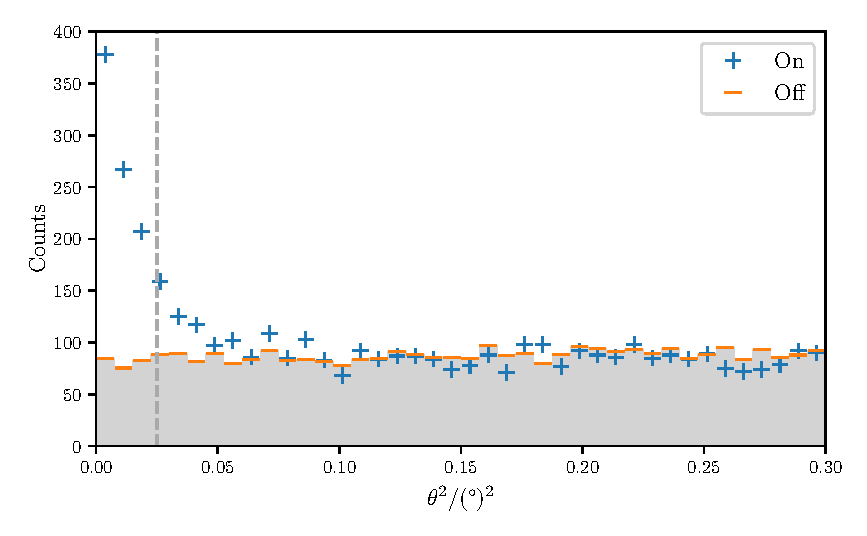
\includegraphics[width=.7\textwidth]{plots/theta_square.pdf}
  \caption{Distribution of events as a function of the squared distance for the on-region (blue) and off-region (orange).}
  \label{fig:theta2}
\end{figure}

In \autoref{fig:theta2} the number of events in dependence of the distance $\theta$ squared to the on and off positions is shown. For the off-event distribution the contributions of each off position are weighted with $0.2$ to allow a comparison of on- and off-event distribution. It is observed, that the off-event distribution is rather isotropic while a large excess of on-events is observed for a small value of $\theta^2$. This motivates the rejection of events with $\theta^2 \leq \num{0.025}$ to reject background. The detection significance of the recorded events below that cut is
\begin{equation}
  S = \num{26.28}. % 26.27587
\end{equation}

\subsection{Energy Migration}

\begin{figure}[tb]
  \centering
  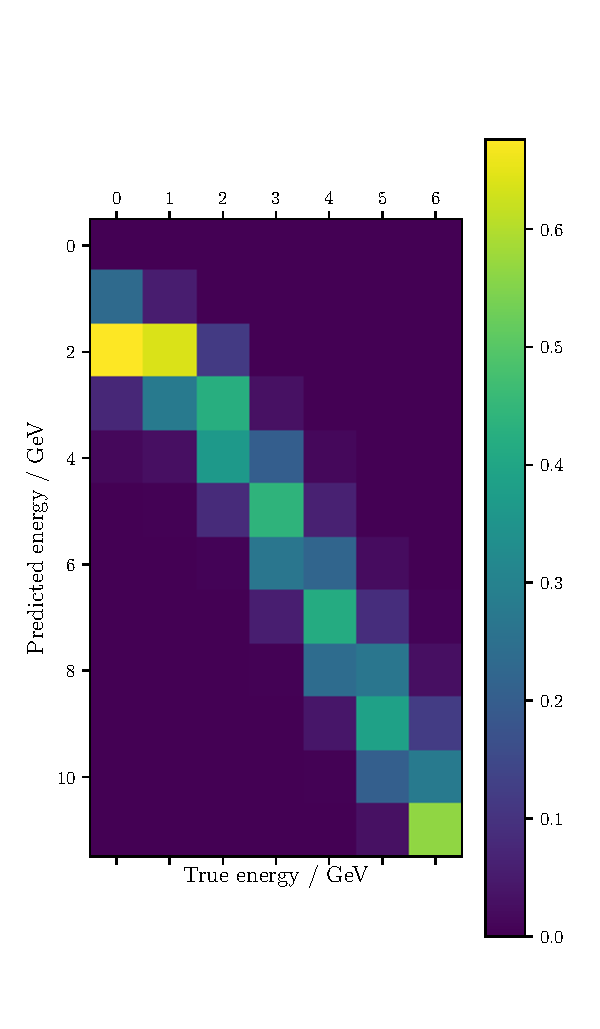
\includegraphics[width=.7\textwidth]{plots/Matrix.pdf}
  \caption{Energy migration matrix of the random-forest regressor.}
  \label{fig:matrix}
\end{figure}

The migration matrix is calculated from the simulation's predicted gamma energy \texttt{gamma\_energy\_prediction} and true energy \texttt{corsika\_event\_header\_total\_energy}. The binning ranges from $\SI{500}{\giga\eV}$ to $\SI{15}{\tera\eV}$. Since inverse problems are often better conditioned when there are more bins in the measured than in the unfolded parameter, $\num{10}$ bins have been chosen for the predicted energy and $\num{5}$ bins have been chosen for the true energy. To take events into account that are not in the chosen energy range, there are also overflow and underflow bins for the predicted and true energy. The migration matrix is visualised in \autoref{fig:matrix}. It can be seen that predicted and true energy are highly correlated.

\subsection{Unfolding}

\begin{figure}[tb]
  \centering
  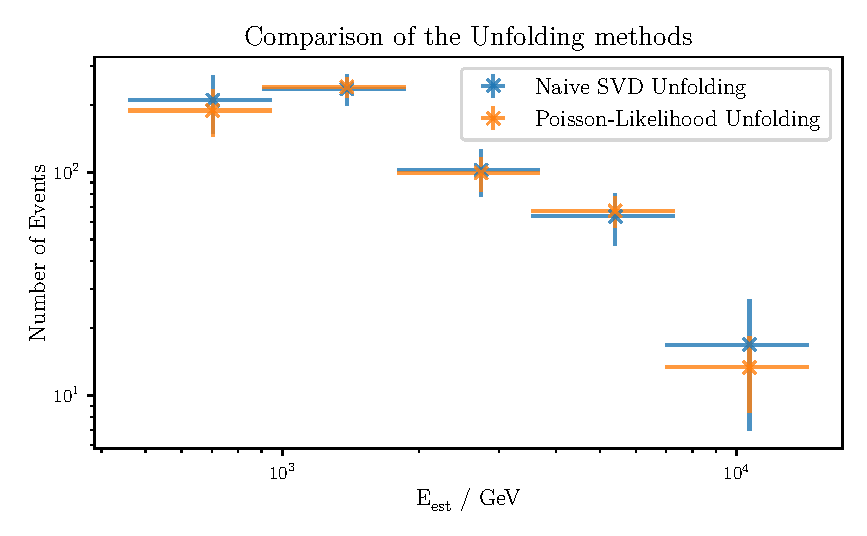
\includegraphics[width=.7\textwidth]{plots/Unfolding_compare.pdf}
  \caption{Unfolded gamma energies in logarithmic bins determined with Naive SVD (blue) and Poisson-Likelihood (orange) unfolding.}
  \label{fig:unfold}
\end{figure}

The measurements are unfolded with the naive SVD method and the Poisson-Likelihood method. The off-events are interpreted as background and the on-events are the desired signal.

For the naive SVD method, the inverse of the migration matrix is needed. Since the energy migration matrix is not a square matrix, the Moore-Penrose-pseudoinverse matrix is calculated using the \texttt{numpy.linalg.pinv} method. Afterwards, the measurement is unfolded as described in \autoref{subsec:Decon} which gives
\begin{equation}
  \hat{\vec{f}}_\mathrm{NSVD} = \begin{pmatrix} \num{210.96 \pm 60.97} \\ \num{236.88 \pm 36.72} \\ \num{102.31 \pm 24.21} \\ \num{63.54 \pm 16.54} \\ \num{16.88 \pm 9.94} \end{pmatrix}.
\end{equation}


For the Poisson-Likelihood unfolding the negative Log-Likelihood is minimised with the \texttt{scipy.optimize.minimize} method. With this method, the unfolded values are found to be
\begin{equation}
  \hat{\vec{f}}_\mathrm{Poisson} = \begin{pmatrix} \num{189.49 \pm 44.80} \\ \num{242.15 \pm 24.67} \\ \num{99.44 \pm 17.05} \\ \num{67.23 \pm 16.54} \\ \num{13.37 \pm 5.02} \end{pmatrix}.
\end{equation}
The results of both methods are visualised in \autoref{fig:unfold}. It can be seen that the results of both methods are well in agreement within their uncertainties.

\subsection{Flux Calculation}

\begin{figure}[tb]
  \centering
  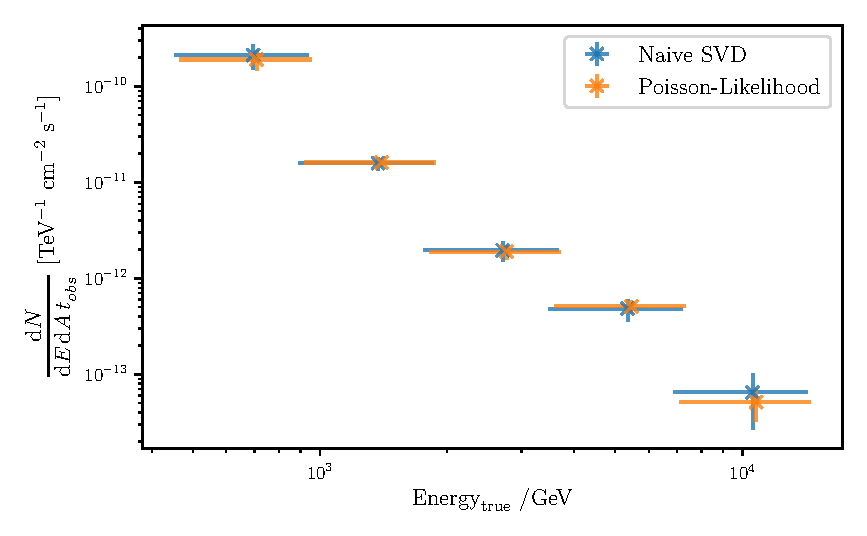
\includegraphics[width=.7\textwidth]{plots/flux.pdf}
  \caption{Flux determined with Naive SVD (blue) and Poisson-Likelihood (orange) unfolding.}
  \label{fig:flux}
\end{figure}

The flux is calculated as described in \autoref{subsec:flux}. To account the fact that the simulated data is only a subset with $\SI{70}{\percent}$ of the originally simulated events, the effective detection area is divided by $\num{0.7}$.
The results for both methods are
\begin{align}
  \Phi_\mathrm{NSVD} = \begin{pmatrix} \num{2.12 \pm .61e-10} \\ \num{1.58 \pm .24e-11} \\ \num{1.95 \pm .46e-12} \\ \num{4.83 \pm 1.26e-13} \\ \num{6.49 \pm 3.82e-14} \end{pmatrix}\,\si{\per\tera\eV\per\cm\squared\per\second} &&  \Phi_\mathrm{Poisson} = \begin{pmatrix} \num{1.90 \pm .45e-10} \\ \num{1.61 \pm .16e-11} \\ \num{1.90 \pm .33e-12} \\ \num{5.11 \pm .82e-13} \\ \num{5.14 \pm 1.93e-14} \end{pmatrix}\,\si{\per\tera\eV\per\cm\squared\per\second}.
\end{align}
The results for both methods are also shown in \autoref{fig:flux}.

\subsection{Comparison with MAGIC and HEGRA}
The flux of the Crab Nebula has also been studied by the HEGRA~\cite{HEGRA} and MAGIC~\cite{MAGIC} collaborations.
These have used a fitting function
\begin{equation}
  f \left( x,a,b,c,d \right) = a \left( \frac{x}{b} \right)^{-c + d \mathrm{ln}\left( \frac{x}{b} \right)}.
\end{equation}
The parameters for both measurements can be taken from \autoref{tab:meas}.

\begin{table}[tb]
  \centering
  \caption{Fitting parameters for the gamma flux from the Crab Nebula of the HEGRA and MAGIC experiments.}
  \begin{tabular}{l l l l l}
    Experiment & $a$/$10^{-11}\,\si{\per\tera\eV\per\cm\squared}$ & $b$/$\si{\tera\eV}$  & $c$ & $d$ \\
    MAGIC & $\num{3.23 \pm .03}$ & $\num{1}$ & $\num{2.47 \pm .01}$ & $\num{-0.24 \pm .01}$ \\
    HEGRA & $\num{2.83 \pm .6}$ & $\num{1}$ & $\num{2.62 \pm .05}$ & $\num{0 \pm 0}$ \\
  \end{tabular}
  \label{tab:meas}
\end{table}
The results of the two experiments as well as the results of this analysis are shown in \autoref{fig:flux_compare}. The results from this analysis are well in agreement with the results from the two collaborations within the uncertainties at energies above $\SI{1}{\tera\eV}$ while the results from this analysis diverge at lower energy.

\begin{figure}[tb]
  \centering
  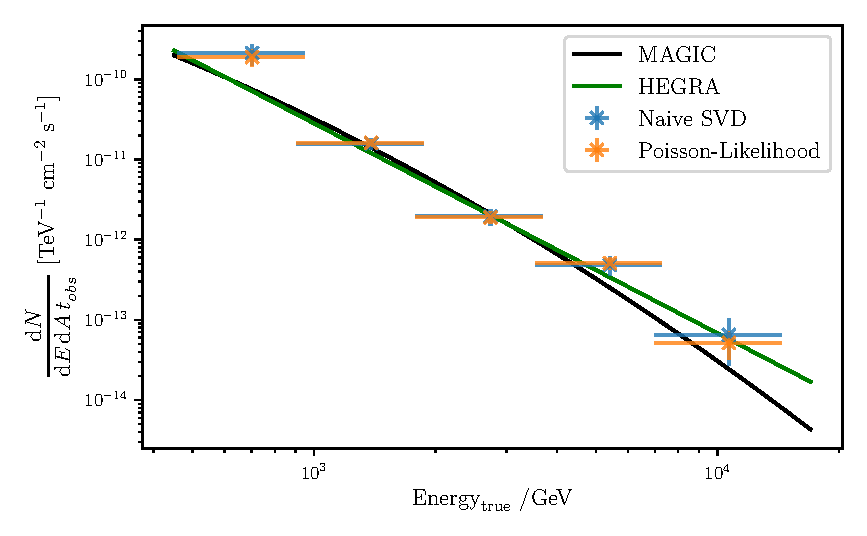
\includegraphics[width=.7\textwidth]{plots/flux_compare.pdf}
  \caption{Calculated flux in this analysis via Naive SVD and Poisson-Likelihood unfolding in comparison to the results of the HEGRA and MAGIC experiments.}
  \label{fig:flux_compare}
\end{figure}
